\section{什么是计算思维？}

计算思维是一种人类的思维过程，是每个人必须掌握的技能。与“听说读写”能力一样，是人类基本思维方式。计算思维不仅仅属于计算机科学家，而是属于每一个人。

\subsection{思考，创新，创造}

当今世界已然是科技驱动的社会。谁拥有核心科技硬实力，谁就能掌握主动。从国家到个人，均无例外。以往教学的重点常常集中于如何让学生理解、记忆现有的体系知识。而世界信息体系发生了变化，我们的教学不可一成不变，也应该随之变化。不能再只是让孩子们了解已有的这些信息（数据），而应该教会他们分析、处理及展示这些信息（数据），把它们真正地用起来。如今的孩子们不应该再过多地死记硬背已有的知识，而应更多的去思考，去创新，去创造。孩子们要\cmagenta{避免形成思维定势，多锻炼将所学应用到现实世界的问题中的能力。}

\subsection{菜谱}

人们在日常生活中的很多做法其实都和计算思维不谋而合，也可以说计算思维从生活中吸收了很多有用的思想和方法。我们来看一些例子。 

算法过程：菜谱可以说是算法（或程序）的典型代表，它将一道菜的烹饪方法一步一步地罗列出来，即使不是专业厨师，照着菜谱的步骤也能做出可口的菜肴。这里，菜谱的每一步骤必须足够简单、可行。例如：“将土豆切成块状”、“将 1 两油入锅加热”等都是可行的步 骤，而“使菜肴具有神秘香味”则不是可行的。

模块化：很多菜谱都有“勾芡”这个步骤，与其说这是一个基本步骤，不如说是一个模块，因为勾芡本身代表着一个操作序列——取一些淀粉，加点水，搅拌均匀，在适当时候倒入菜中。由于这个操作序列经常使用，为了避免重复，也为了使菜谱结构清晰、易读，所以 用“勾芡”这个术语简明地表示。这个例子同时也反映了在不同层次上进行抽象的思想。

并发。厨师在烧菜时，如果一个菜需要在锅中煮一段时间，厨师一定会利用这段时间去做点别的事情（比如将另一个菜洗净切好），而绝不会无所事事。在此期间如果锅里的菜需要 加盐加佐料，厨师可以放下手头的活儿去处理锅里的菜。就这样，虽然只有一个厨师，但他可以同时做几个菜。

\subsection{求解问题中的计算思维}

利用计算手段求解问题的过程是：首先要把实际的应用问题转换为数学问题，可能是一组偏微分方程，其次将PDE离散为一组代数方程组，然后建立模型、设计算法和编程实现，最后在实际的计算机中运行并求解。前两步是计算思维中的抽象，后两步是计算思维中的自动化。

\subsection{系统设计中的计算思维}

R.Karp：任何自然系统和社会系统都可视为一个动态演化系统，演化伴随着物质、能量和信息的交换，这种交换可以映射为符号变换，使之能用计算机进行离散的符号处理。

当动态演化系统抽象为离散符号系统后，就可以采用形式化的规范描述，建立模型、设计算法和开发软件来揭示演化的规律，实时控制系统的演化并自动执行。

\subsection{人类行为理解中的计算思维}

利用计算手段来研究人类的行为，可视为社会计算，即通过各种信息技术手段，设计、实施和评估人与环境之间的交互。

\section{计算思维的本质}

Abstraction （抽象）和Automation（自动化）是计算思维的两大核心特征。

\begin{enumerate}
    \item 把实际问题抽象为数学问题，并建模
    
    将人对问题的理解用数学语言描述出来
    \item 进行映射，把数学模型中的变量等用特定的符号代替
    
    用符号一一对应数学模型中的变量和规则等
    \item 通过编程把解决问题的逻辑分析过程写成算法
    
    把解题思路变成计算机指令，也就是算法
    \item 执行算法，进行求解
    
    计算机根据算法，一步步完成相应指令，求出结果
\end{enumerate}

建立数学模型的过程就是理解问题的过程，并且要把你对问题的理解用数学语言描述出来。这很关键，数学模型的好坏意味着你对问题的理解程度够不够深，而且数学模型还说明了在这个问题中，哪些东西可以计算以及如何进行计算，这可以说是计算思维里最最核心的东西了。这个关键过程需要的核心能力就是抽象能力以及一定的数学基础。

数学建模只是可计算化的第一步，为了让计算机帮我们去求解，我们还需要虚拟的符号来代替的数学模型里的每个变量和运算规则，这个过程就是映射啦！

完成映射，我们就能把解题思路（注意，是解题思路，不是数学模型）用程序语言完整地告诉计算机啦，这个过程就是具体的编程写算法的过程啦！这一步需要较强的编程能力，但编程能力的核心之一也是抽象思维能力。对于编程能力不够强的人来说，映射还有编程的过程可以交给擅长编程的人来做。

关键路径的前3步都是人来完成的，最后一步执行算法进行运算是机器自动完成的，体现了计算思维的自动化的特点。

在整个过程中，抽象是方法，是手段，贯穿整个过程的每个环节。自动化是最终目标，让机器去做计算的工作，把人脑解放出来，中间目标是实现问题的可计算化，体现在成果上就是数学模型、映射、还有算法。


\subsection{理解计算思维，首先要理解计算}

理解计算思维的前提是理解计算，因为计算思维本质上还是研究计算的，研究在解决问题过程中，哪些是可计算的，以及如何计算。

通常我们理解的计算是算术运算，如“1+1=2”，，但运算其实有很多种类，如集合运算、逻辑运算、条件运算等等。集合运算这里面就没有具体的数值运算了，而是用代表集合的字母进行运算；又比如逻辑运算“1∧0=0”，这个运算里有数值“0”和1，但意义完全不同，这里的“1”代表的是“真”—即命题为真，“0”代表的是“假”—即命题为假，通过用数字“0”和“1”来代换命题的真假，用“∧”来代换逻辑语言里的“并且”，逻辑判断过程也能通过计算来实现。

当我们跳出算术运算的局限，理解了计算的本质后，就会发现原来好多看似不可计算的东西都能变得可计算，也就很容易理解计算思维的普适性了。因为经过一定的抽象，我们对很多问题的理解都能用特定的数学语言来描述，接下来，当我们用特定的数学语言去描述解决过程的时候，就是在用计算化的方式来求解了。

\subsection{抽象}

在哥尼斯堡城的普莱格尔河上有7座桥，将河中的两个岛和河岸连结问能否一次走遍7座桥，而每座桥只允许通过一次，最后仍然回到起始地点。

1736年29岁的欧拉向圣彼得堡科学院递交了《哥尼斯堡的七座桥》的论文，在解答问题的同时，开创了数学的一个新的分支——图论与几何拓扑，也由此展开了数学史上的新历程。

大数学家欧拉把它转化成一个几何问题——一笔画问题。他不仅解决了此问题，且给出了连通图可以一笔画的充要条件是：奇点的数目不是0个就是2个（连到一点的数目如果是奇数条，就称为奇点；如果是偶数条，就称为偶点。要想一笔画成，必须中间点均是偶点，也就是有来路必有另一条去路，奇点只可能在两端。因此任何图能一笔画成，奇点要么没有，要么在两端）

\section{计算思维对其他学科的影响}

\subsection{人类基因组计划}

人类基因组计划（英语：Human Genome Project, HGP）是一项规模高，跨国跨学科的科学探索巨型工程。其宗旨在于测定组成人类染色体（指单倍体）中所包含的六十亿对组成的核苷酸序列，从而绘制人类基因组图谱，并且辨识其载有的基因及其序列，达到破译人类遗传信息的最终目的。基因组计划是人类为了探索自身的奥秘所迈出的重要一步。截至2005年，人类基因组计划的测序工作已经基本完成（92\%）。其中，2001年人类基因组工作草图的发表（由公共基金资助的国际人类基因组计划和私人企业塞雷拉基因组公司各自独立完成，并分别公开发表）被认为是人类基因组计划成功的里程碑。

\subsection{霰弹枪测序法}

霰弹枪定序法（又称鸟枪法）是一种广泛使用的为长DNA测序的方法，比传统的定序法快速，但精确度较差。曾经使用于塞雷拉基因组（Celera Genomics）公司所主持的人类基因组计划。

霰弹枪测序法的思想是将基因组打断为数百万个DNA片断，然后用一定的算法将片断的序列信息重新整合在一起，从而得到整个基因组序列。为了提高这一方法的效率，1980年代，测序和片断信息整合达到了自动化。这一方法虽然已被用于序列长达6百万个碱基对的细菌基因组测序，但对于人类基因组中3千万个碱基对的序列测定，这一技术能否成功在当时还未有定论。

\section{算法的表示}

\subsection{自然语言表示}

用自然语言来描述算法。

使用自然语言描述算法的优点是通俗易懂。但是，自然语言本身所固有的不严密性使得这种描述方法存在“文字冗长，容易产生歧义性”以及“难以描述算法中的分支和循环等结构”等缺陷。

\subsection{流程图}

流程图是一种传统的、广泛应用的算法描述工具，也是最常见的算法图形化表达工具。

流程图利用几何图形的图框来代表各种不同的操作，用流程线来指示算法的执行方向，它使用规定的一些图框、线条来形象、直观地描述算法处理过程。

与自然语言相比，流程图可以清晰、直观、形象地反应控制结构的过程。

\begin{figure}[htpb]
    \centering
    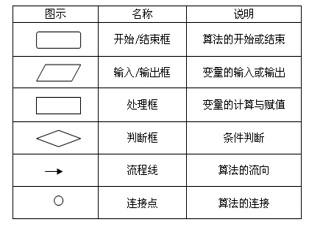
\includegraphics[width=.5\linewidth]{figures/flowchart.jpg}
\end{figure}

\cred{为什么使用变量？}

存放数据。

算法中的初始数据、计算的中间结果和最后结果都需要存放到变量中。

\cred{如何在变量中存入数据？}
\begin{itemize}
    \item 赋值
    \item 输入
\end{itemize}

大多算法和编程语言使用等号=表示赋值操作，称为赋值号。等号在算法中表示的是赋值，不是相等。

\begin{framed}
例如：

$a=5$

$a=a+3$

如果表示数学上的等于，这是不合理的！而算法中表示的是赋值：先计算加，读取a的值5加3得8，然后将8赋值给a，a的值变为8。

每次对变量赋值时，新值会覆盖掉变量中原来存放的值。所以在一段时间中变量的值是变化的，但在任一时刻只对应一个值。
\end{framed}


